\documentclass[../../main]{subfiles}
\begin{document}
\section{Hierarchical clustering}
\label{ch:results_rq1}
In the this section we present the results of the experiment with hierarchical clustering.
We divide the results in two variants. 
The first variant displays the results of clustering with all characteristics.
The second variant displays the results of clustering without the Levensthein distance.
\newline
For each variant and project we display the weighted mutation score to create box-plots.
There are a total of eleven projects and thus also eleven box-plots per variant.
In a box-plot the box is from the first quartile till the third quartile and a line at the median. 
The dots are measurement points laying outside the fences, which are located at Q1  1.5(Q3  Q1) and Q3+1.5(Q3  Q1). 
The whiskers show the range of points that are outside the box but inside the fences.
\newline
Due to the limitation of resources and time we had to omit four source projects from these results. 
The hardware was not equipped to store the amount of generated mutants for these projects, we did not have enough memory.
Trying to cluster these mutants this resulted in a out of memory error.
\newline
The results displayed are the average of the results of the 30 repetitions of the experiment.
The result of each single repetition can be found in our Github repository\cite{rbasarat-repo}.

\subsection{Clustering with all characteristics}
This section displays the results of our clustering algorithm when executed with data that consists of all characteristics.
The results are be grouped based on the percentage in reduction of mutants executed.
We also display the accuracy of the clusters per reduction.
The results displayed are the average of the results of the 30 repetitions of the experiment.
The result of each single repetition can be found in our Github repository\cite{rbasarat-repo}.

\begin{figure}[H]
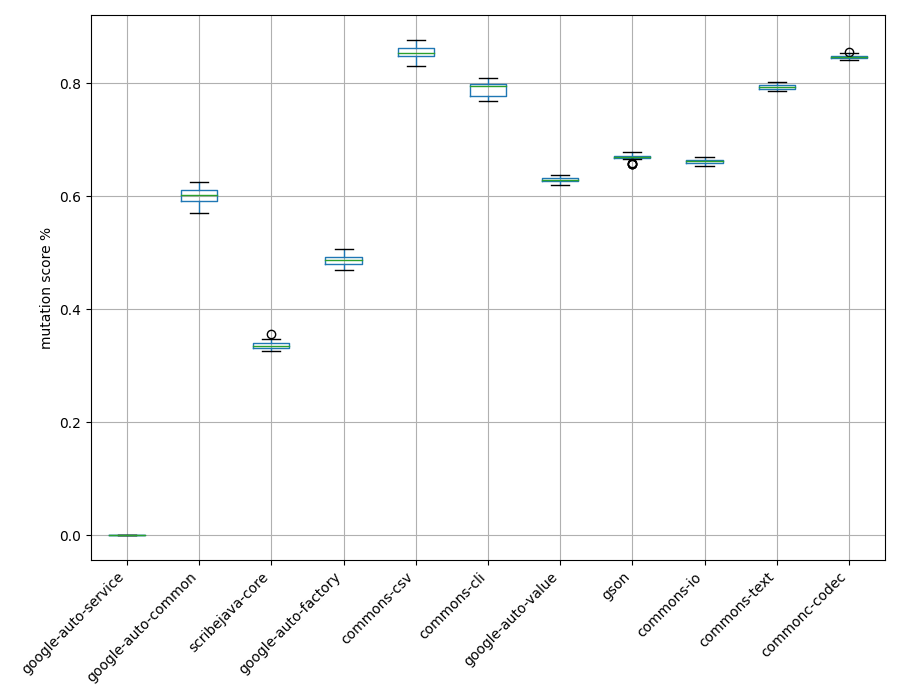
\includegraphics[width=\textwidth]{images/boxplot_summary/boxplot_hc_full_0.25.png}
\caption{\label{box:clustering_all_25}Box-plots containing weighted mutation score of clustering mutants with all characteristics and cluster size of n*0.25}
\end{figure}


\begin{table}[!htb]
\begin{tabular}{|l|c|c|c|c|c|}
\hline
\multicolumn{1}{|c|}{Project} & \begin{tabular}[c]{@{}c@{}}Mutation score\\ full set\end{tabular} & \begin{tabular}[c]{@{}c@{}}Mutation score \\ clustered set\end{tabular} & \begin{tabular}[c]{@{}c@{}}Avg. cluster\\  accuracy\end{tabular} & \begin{tabular}[c]{@{}c@{}}Min. cluster\\ accuracy\end{tabular} & \begin{tabular}[c]{@{}c@{}}Max. cluster\\ accuracy\end{tabular} \\ \hline
Google Auto Service           & 0.00\%                                                                                  & 0.00\%                                                                                      & 0.00\%                                                                               & 0.00\%                                                                                & 0.00\%                                                                               \\ \hline
ScribeJava-Core               & 33.52\%                                                                                 & 33.63\%                                                                                     & 93.29\%                                                                              & 50.00\%                                                                               & 100.00\%                                                                             \\ \hline
Google Auto Factory           & 48.41\%                                                                                 & 48.58\%                                                                                     & 94.18\%                                                                              & 50.00\%                                                                               & 100.00\%                                                                             \\ \hline
Google Auto Common            & 59.59\%                                                                                 & 60.14\%                                                                                     & 91.12\%                                                                              & 50.00\%                                                                               & 100.00\%                                                                             \\ \hline
Google Auto Value             & 61.42\%                                                                                 & 62.89\%                                                                                     & 94.33\%                                                                              & 50.00\%                                                                               & 100.00\%                                                                             \\ \hline
Google Gson                   & 66.83\%                                                                                 & 66.87\%                                                                                     & 91.61\%                                                                              & 50.00\%                                                                               & 100.00\%                                                                             \\ \hline
commons-io                    & 69.70\%                                                                                 & 66.18\%                                                                                     & 90.36\%                                                                              & 50.00\%                                                                               & 100.00\%                                                                             \\ \hline
commons-cli                   & 79.07\%                                                                                 & 79.01\%                                                                                     & 91.35\%                                                                              & 50.00\%                                                                               & 100.00\%                                                                             \\ \hline
commons-text                  & 79.29\%                                                                                 & 79.33\%                                                                                     & 89.95\%                                                                              & 50.00\%                                                                               & 100.00\%                                                                             \\ \hline
commons-codec                 & 84.56\%                                                                                 & 84.71\%                                                                                     & 94.44\%                                                                              & 50.00\%                                                                               & 100.00\%                                                                             \\ \hline
commons-csv                   & 85.16\%                                                                                 & 85.42\%                                                                                     & 92.08\%                                                                              & 50.00\%                                                                               & 100.00\%                                                                             \\ \hline

\end{tabular}
\caption{\label{tab:clustering_all_25}Results of clustering mutants with all characteristics and cluster size of n*0.25}
\end{table}
\FloatBarrier

Figure \ref{box:clustering_all_25} displays the box-plots of the weighted mutation score obtained from each individual sample. 
We can observe that for every box-plot the \textit{p-value} is below 0.05 or 5\%.
To view the box-plots separately and in more detail see Appendix \ref{ap:full_25}.
Table \ref{tab:clustering_all_25} displays the results of clustering mutants with all characteristics and the number of clusters equal to the total amount of mutants* 0.25.  
The maximum and minimum differences between the score of a full set and clustered are is 3.52\% and 0.04\% respectively.  
The average of the differences between full set score and clustered score is 0.58\%.
It is also noticeable that the minimum and maximum accuracy are 50\% and 100\% respectively.
This means that there was at least one cluster that consisted of only mutants that were killed or survived.
The minimum accuracy cannot go below 50\%.
If the percentage does go below 50\% the representation of a cluster will flip from survived to killed or the other way around.

\begin{figure}[H]
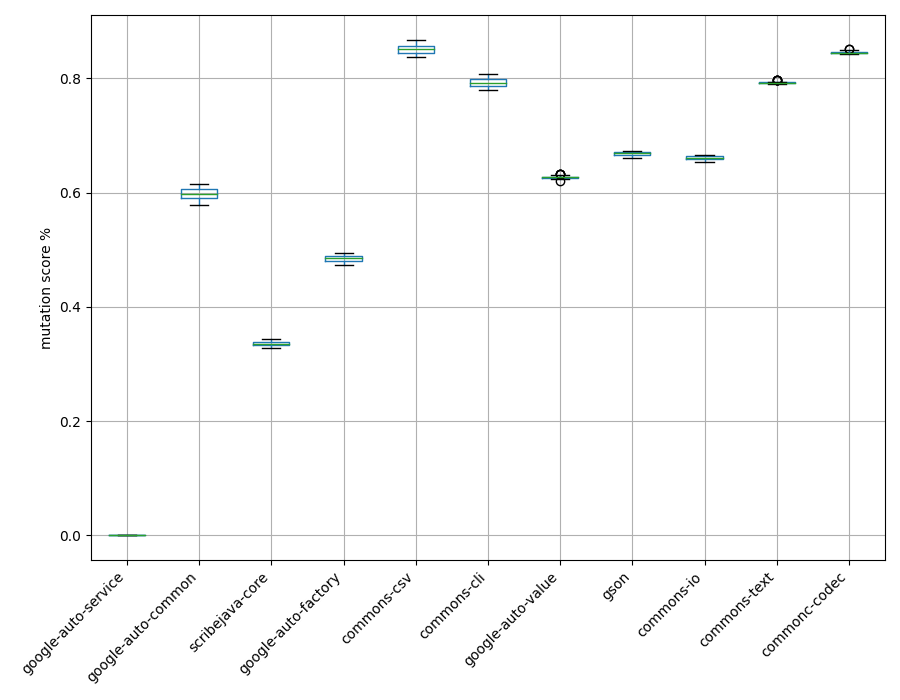
\includegraphics[width=\textwidth]{images/boxplot_summary/boxplot_hc_full_0.5.png}
\caption{\label{box:clustering_all_50}Box-plots containing weighted mutation score of clustering mutants with all characteristics and cluster size of n*0.5}
\end{figure}

\begin{table}[!htb]
\begin{tabular}{|l|c|c|c|c|c|}
\hline
\multicolumn{1}{|c|}{Project} & \begin{tabular}[c]{@{}c@{}}Mutation score\\ full set\end{tabular} & \begin{tabular}[c]{@{}c@{}}Mutation score \\ clustered set\end{tabular} & \begin{tabular}[c]{@{}c@{}}Avg. cluster\\  accuracy\end{tabular} & \begin{tabular}[c]{@{}c@{}}Min. cluster\\ accuracy\end{tabular} & \begin{tabular}[c]{@{}c@{}}Max. cluster\\ accuracy\end{tabular} \\ \hline
Google Auto Service           & 0.00\%                                                                                  & 0.00\%                                                                                      & 0.00\%                                                                               & 0.00\%                                                                                & 0.00\%                                                                             \\ \hline
ScribeJava-Core               & 33.52\%                                                                                 & 33.54\%                                                                                     & 96.94\%                                                                              & 50.00\%                                                                               & 100.00\%                                                                             \\ \hline
Google Auto Factory           & 48.41\%                                                                                 & 48.39\%                                                                                     & 96.12\%                                                                              & 50.00\%                                                                               & 100.00\%                                                                             \\ \hline
Google Auto Common            & 59.59\%                                                                                 & 59.76\%                                                                                     & 94.49\%                                                                              & 50.00\%                                                                               & 100.00\%                                                                             \\ \hline
Google Auto Value             & 61.42\%                                                                                 & 62.71\%                                                                                     & 96.09\%                                                                              & 50.00\%                                                                               & 100.00\%                                                                             \\ \hline
Google Gson                   & 66.83\%                                                                                 & 66.81\%                                                                                     & 94.75\%                                                                              & 50.00\%                                                                               & 100.00\%                                                                             \\ \hline
commons-io                    & 69.70\%                                                                                 & 66.06\%                                                                                     & 94.03\%                                                                              & 50.00\%                                                                               & 100.00\%                                                                             \\ \hline
commons-cli                   & 79.07\%                                                                                 & 79.17\%                                                                                     & 94.19\%                                                                              & 50.00\%                                                                               & 100.00\%                                                                             \\ \hline
commons-text                  & 79.29\%                                                                                 & 79.29\%                                                                                     & 93.21\%                                                                              & 50.00\%                                                                               & 100.00\%                                                                             \\ \hline
commons-codec                 & 84.56\%                                                                                 & 84.60\%                                                                                     & 95.92\%                                                                              & 50.00\%                                                                               & 100.00\%                                                                             \\ \hline
commons-csv                   & 85.16\%                                                                                 & 85.13\%                                                                                     & 94.65\%                                                                              & 50.00\%                                                                               & 100.00\%                                                                             \\ \hline
\end{tabular}
\caption{\label{tab:clustering_all_50}Results of clustering mutants with all characteristics and size n*0.50}
\end{table}
\FloatBarrier

Figure \ref{box:clustering_all_50} displays the box-plots of the weighted mutation score obtained from each individual sample. 
We can observe that for every box-plot the \textit{p-value} is below 0.05 or 5\%.
To view the box-plots separately and in more detail see Appendix \ref{ap:full_50}.
Table \ref{tab:clustering_all_50} displays the results of clustering mutants with all characteristics and the number of clusters equal to the total amount of mutants* 0.50.  
The maximum and minimum differences between the score of a full set and clustered set are 3.63\% and 0.02\% respectively.
The average of the differences between full set score and clustered score is 0.48\% which is smaller than the average difference than that of the 25\% set.

\begin{figure}[H]
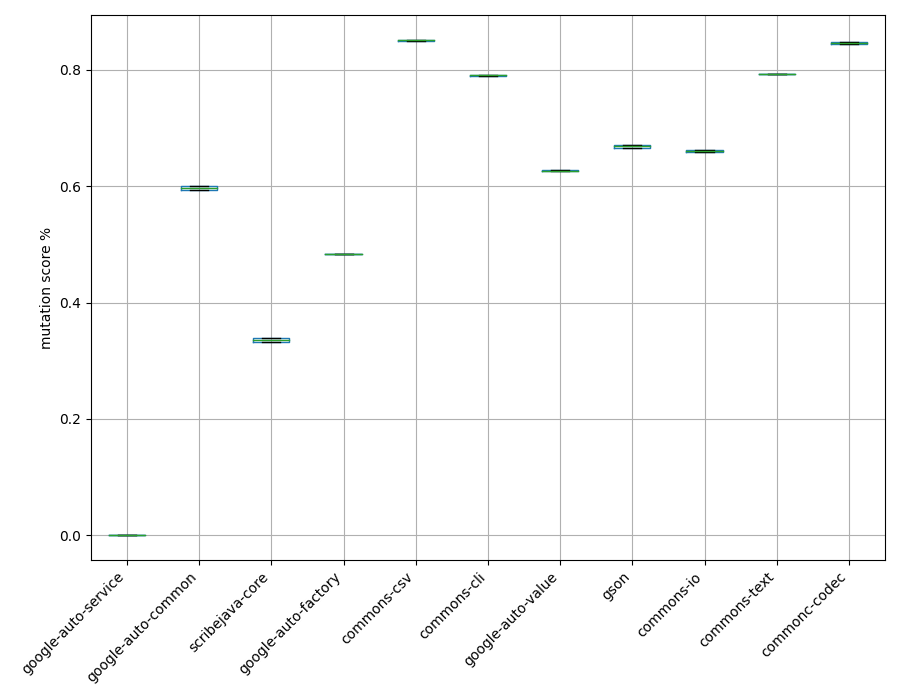
\includegraphics[width=\textwidth]{images/boxplot_summary/boxplot_hc_full_0.75.png}
\caption{\label{box:clustering_all_75}Box-plots containing weighted mutation score of clustering mutants with all characteristics and cluster size of n*0.75}
\end{figure}

\begin{table}[!htb]
\begin{tabular}{|l|c|c|c|c|c|}
\hline
\multicolumn{1}{|c|}{Project} & \begin{tabular}[c]{@{}c@{}}Mutation score\\ full set\end{tabular} & \begin{tabular}[c]{@{}c@{}}Mutation score \\ clustered set\end{tabular} & \begin{tabular}[c]{@{}c@{}}Avg. cluster\\  accuracy\end{tabular} & \begin{tabular}[c]{@{}c@{}}Min. cluster\\ accuracy\end{tabular} & \begin{tabular}[c]{@{}c@{}}Max. cluster\\ accuracy\end{tabular} \\ \hline
Google Auto Service           & 0.00\%                                                                                  & 0.00\%                                                                                      & 0.00\%                                                                               & 0.00\%                                                                                & 0.00\%                                                                               \\ \hline
ScribeJava-Core               & 33.52\%                                                                                 & 33.52\%                                                                                     & 97.99\%                                                                              & 50.00\%                                                                               & 100.00\%                                                                             \\ \hline
Google Auto Factory           & 48.41\%                                                                                 & 48.41\%                                                                                     & 97.46\%                                                                              & 50.00\%                                                                               & 100.00\%                                                                             \\ \hline
Google Auto Common            & 59.59\%                                                                                 & 59.76\%                                                                                     & 96.16\%                                                                              & 50.00\%                                                                               & 100.00\%                                                                             \\ \hline
Google Auto Value             & 61.42\%                                                                                 & 62.68\%                                                                                     & 97.31\%                                                                              & 50.00\%                                                                               & 100.00\%                                                                             \\ \hline
Google Gson                   & 66.83\%                                                                                 & 66.84\%                                                                                     & 97.59\%                                                                              & 50.00\%                                                                               & 100.00\%                                                                             \\ \hline
commons-io                    & 69.70\%                                                                                 & 66.07\%                                                                                     & 97.19\%                                                                              & 50.00\%                                                                               & 100.00\%                                                                             \\ \hline
commons-cli                   & 79.07\%                                                                                 & 79.10\%                                                                                     & 96.68\%                                                                              & 50.00\%                                                                               & 100.00\%                                                                             \\ \hline
commons-text                  & 79.29\%                                                                                 & 79.33\%                                                                                     & 97.61\%                                                                              & 50.00\%                                                                               & 100.00\%                                                                             \\ \hline
commons-codec                 & 84.56\%                                                                                 & 84.61\%                                                                                     & 98.84\%                                                                              & 50.00\%                                                                               & 100.00\%                                                                             \\ \hline
commons-csv                   & 85.16\%                                                                                 & 85.07\%                                                                                     & 97.64\%                                                                              & 50.00\%                                                                               & 100.00\%                                                                             \\ \hline
\end{tabular}
\caption{\label{tab:clustering_all_75}Results of clustering mutants with a single characteristic and size n*0.75}
\end{table}
\FloatBarrier

Figure \ref{box:clustering_all_75} displays the box-plots of the weighted mutation score obtained from each individual sample. 
We can observe that for every box-plot the \textit{p-value} is below 0.05 or 5\%.
To view the box-plots separately and in more detail see Appendix \ref{ap:full_75}.
Table \ref{tab:clustering_all_75} displays the results of clustering mutants with all characteristics and the number of clusters equal to the total amount of mutants* 0.75.  
The maximum and minimum differences between the score of a full set and clustered set are 3.63\% and 0\% respectively.  
The average of the differences between full set score and clustered score is 0.48\% which is higher than the average difference than that of the 25\% and the same of that of the 50\% set.

%---------------- from here no levenshtein ---------------------------%

\subsection{Clustering without Levenshtein distance}
This section will display the results of our clustering algorithm when executed without the Levenshtein distance.
The results will be grouped based on the reduced percentage of mutants executed.
We will also display the accuracy of the clusters per reduction amount.
The results displayed are the average of the results of the 30 repetitions of the experiment.
The result of each single repetition can be found in our Github repository\cite{rbasarat-repo}.

\begin{figure}[H]
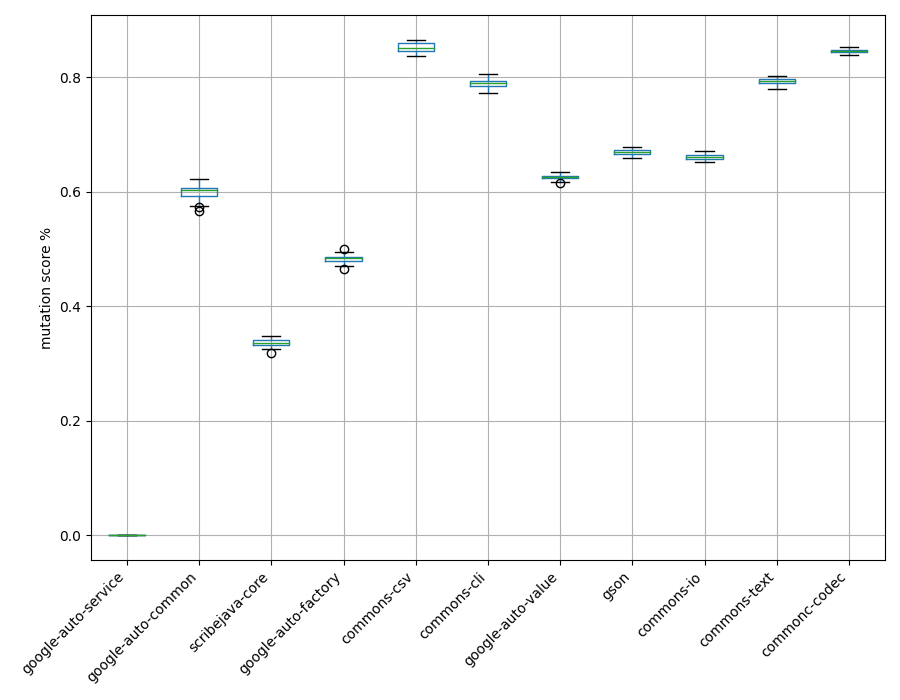
\includegraphics[width=\textwidth]{images/boxplot_summary/boxplot_hc_no_distance_0.25.png}
\caption{\label{box:clustering_no_distance_25}Box-plots containing weighted mutation score of clustering mutants without Levensthein distance and cluster size n*0.25}
\end{figure}

\begin{table}[htb]
\begin{tabular}{|l|c|c|c|c|c|}
\hline
\multicolumn{1}{|c|}{Project} & \begin{tabular}[c]{@{}c@{}}Mutation score\\ full set\end{tabular} & \begin{tabular}[c]{@{}c@{}}Mutation score \\ clustered set\end{tabular} & \begin{tabular}[c]{@{}c@{}}Avg. cluster\\  accuracy\end{tabular} & \begin{tabular}[c]{@{}c@{}}Min. cluster\\ accuracy\end{tabular} & \begin{tabular}[c]{@{}c@{}}Max. cluster\\ accuracy\end{tabular} \\ \hline
Google Auto Service           & 0.00\%                                                                                  & 0.00\%                                                                                      & 0.00\%                                                                               & 0.00\%                                                                                & 0.00\%                                                                               \\ \hline
ScribeJava-Core               & 33.52\%                                                                                 & 33.72\%                                                                                     & 92.24\%                                                                              & 50.00\%                                                                               & 100.00\%                                                                             \\ \hline
Google Auto Factory           & 48.41\%                                                                                 & 48.32\%                                                                                     & 94.21\%                                                                              & 50.00\%                                                                               & 100.00\%                                                                             \\ \hline
Google Auto Common            & 59.59\%                                                                                 & 60.03\%                                                                                     & 91.19\%                                                                              & 50.00\%                                                                               & 100.00\%                                                                             \\ \hline
Google Auto Value             & 61.42\%                                                                                 & 62.58\%                                                                                     & 93.90\%                                                                              & 50.00\%                                                                               & 100.00\%                                                                             \\ \hline
Google Gson                   & 66.83\%                                                                                 & 66.89\%                                                                                     & 91.75\%                                                                              & 50.00\%                                                                               & 100.00\%                                                                             \\ \hline
commons-io                    & 69.70\%                                                                                 & 66.08\%                                                                                     & 90.20\%                                                                              & 50.00\%                                                                               & 100.00\%                                                                             \\ \hline
commons-cli                   & 79.07\%                                                                                 & 78.97\%                                                                                     & 91.11\%                                                                              & 50.00\%                                                                               & 100.00\%                                                                             \\ \hline
commons-text                  & 79.29\%                                                                                 & 79.30\%                                                                                     & 90.95\%                                                                              & 50.00\%                                                                               & 100.00\%                                                                             \\ \hline
commons-codec                 & 84.56\%                                                                                 & 84.59\%                                                                                     & 94.56\%                                                                              & 50.00\%                                                                               & 100.00\%                                                                             \\ \hline
commons-csv                   & 85.16\%                                                                                 & 85.24\%                                                                                     & 92.76\%                                                                              & 50.00\%                                                                               & 100.00\%                                                                             \\ \hline
\end{tabular}
\caption{\label{tab:clustering_no_distance_25}Results of clustering mutants without Levensthein distance and cluster size n*0.25}
\end{table}
\FloatBarrier

Figure \ref{box:clustering_no_distance_25} displays the box-plots of the weighted mutation score obtained from each individual sample.
We can observe that for every box-plot the \textit{p-value} is below 0.05 or 5\%.
To view the box-plots separately and in more detail see Appendix \ref{ap:no_distance_25}.
Table \ref{tab:clustering_no_distance_25} displays the results of clustering mutants without Levensthein distance and the number of clusters equal to the total amount of mutants * 0.25. 
We observe that the maximum and minimum differences in mutation score between a full set and a clustered set  3.61\% and 0.09\% respectively.
The average of the differences between full set score and clustered score is 0.53\%.

\begin{figure}[H]
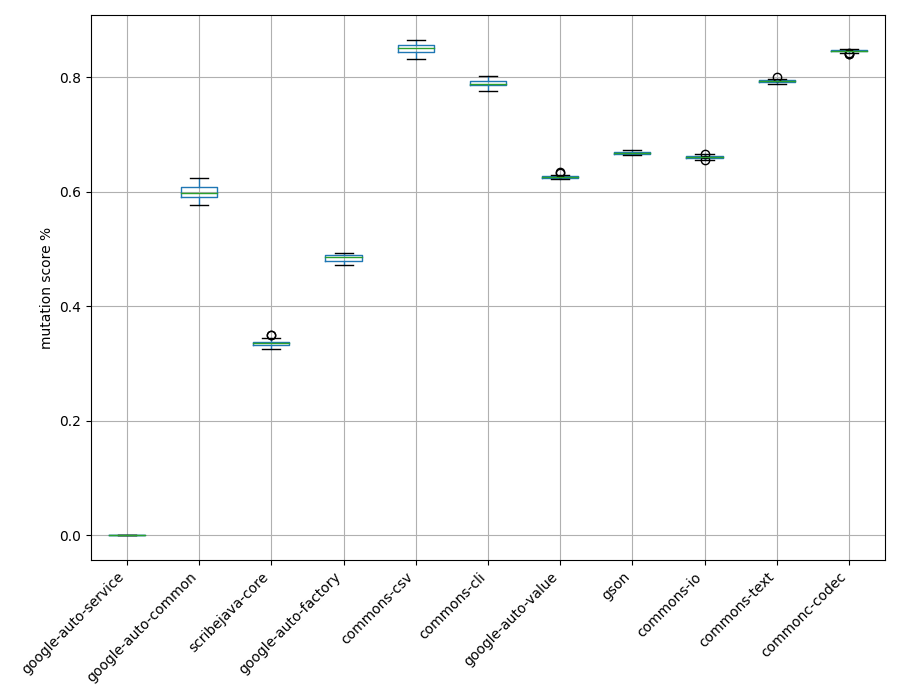
\includegraphics[width=\textwidth]{images/boxplot_summary/boxplot_hc_no_distance_0.5.png}
\caption{\label{box:clustering_no_distance_50}Box-plots containing weighted mutation score of clustering mutants without Levensthein distance and cluster size n*0.50}
\end{figure}

\begin{table}[htb]
\begin{tabular}{|l|c|c|c|c|c|}
\hline
\multicolumn{1}{|c|}{Project} & \begin{tabular}[c]{@{}c@{}}Mutation score\\ full set\end{tabular} & \begin{tabular}[c]{@{}c@{}}Mutation score \\ clustered set\end{tabular} & \begin{tabular}[c]{@{}c@{}}Avg. cluster\\  accuracy\end{tabular} & \begin{tabular}[c]{@{}c@{}}Min. cluster\\ accuracy\end{tabular} & \begin{tabular}[c]{@{}c@{}}Max. cluster\\ accuracy\end{tabular} \\ \hline
Google Auto Service           & 0.00\%                                                                                  & 0.00\%                                                                                      & 0.00\%                                                                               & 0.00\%                                                                                & 0.00\%                                                                               \\ \hline
ScribeJava-Core               & 33.52\%                                                                                 & 33.55\%                                                                                     & 97.16\%                                                                              & 50.00\%                                                                               & 100.00\%                                                                             \\ \hline
Google Auto Factory           & 48.41\%                                                                                 & 48.44\%                                                                                     & 97.71\%                                                                              & 50.00\%                                                                               & 100.00\%                                                                             \\ \hline
Google Auto Common            & 59.59\%                                                                                 & 59.86\%                                                                                     & 96.35\%                                                                              & 50.00\%                                                                               & 100.00\%                                                                             \\ \hline
Google Auto Value             & 61.42\%                                                                                 & 62.62\%                                                                                     & 97.31\%                                                                              & 50.00\%                                                                               & 100.00\%                                                                             \\ \hline
Google Gson                   & 66.83\%                                                                                 & 66.81\%                                                                                     & 95.29\%                                                                              & 50.00\%                                                                               & 100.00\%                                                                             \\ \hline
commons-io                    & 69.70\%                                                                                 & 66.05\%                                                                                     & 95.08\%                                                                              & 50.00\%                                                                               & 100.00\%                                                                             \\ \hline
commons-cli                   & 79.07\%                                                                                 & 78.97\%                                                                                     & 95.55\%                                                                              & 50.00\%                                                                               & 100.00\%                                                                             \\ \hline
commons-text                  & 79.29\%                                                                                 & 79.30\%                                                                                     & 95.34\%                                                                              & 50.00\%                                                                               & 100.00\%                                                                             \\ \hline
commons-codec                 & 84.56\%                                                                                 & 84.59\%                                                                                     & 96.95\%                                                                              & 50.00\%                                                                               & 100.00\%                                                                             \\ \hline
commons-csv                   & 85.16\%                                                                                 & 85.11\%                                                                                     & 95.87\%                                                                              & 50.00\%                                                                               & 100.00\%                                                                             \\ \hline
\end{tabular}
\caption{\label{tab:clustering_no_distance_50}Results of clustering mutants without Levensthein distance and cluster size n*0.50}
\end{table}
\FloatBarrier

Figure \ref{box:clustering_no_distance_50} displays the box-plots of the weighted mutation score obtained from each individual sample. 
We can observe that for every box-plot the \textit{p-value} is below 0.05 or 5\%.
To view the box-plots separately and in more detail see Appendix \ref{ap:no_distance_50}.
Table \ref{tab:clustering_no_distance_50} displays the results of clustering mutants without Levensthein distance and the number of clusters equal to the total amount of mutants * 0.50.
The maximum and minimum differences between the score of a full set and clustered set are 3.65\% and 0.03\% respectively.
We observe that the average cluster accuracy is higher than the average cluster accuracy of the 25\% set. 
The average of the differences between full set score and clustered score is 0.49\% which is smaller than the average difference than that of the 25\% set.

\begin{figure}[H]
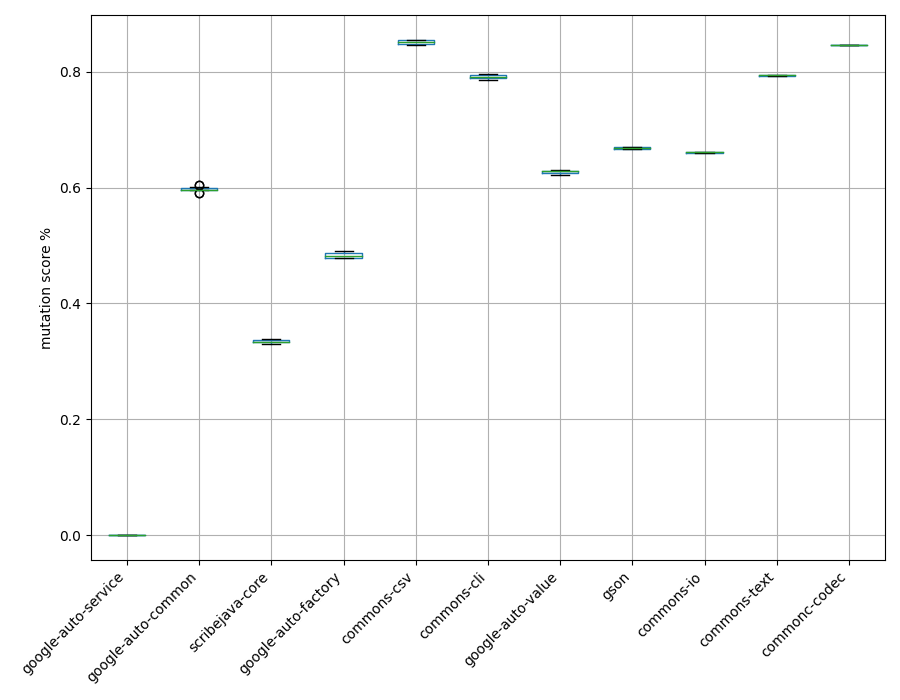
\includegraphics[width=\textwidth]{images/boxplot_summary/boxplot_hc_no_distance_0.75.png}
\caption{\label{box:clustering_no_distance_75}Box-plots containing weighted mutation score of clustering mutants without Levensthein distance and cluster size n*0.75}
\end{figure}

\begin{table}[htb]
\begin{tabular}{|l|c|c|c|c|c|}
\hline
\multicolumn{1}{|c|}{Project} & \begin{tabular}[c]{@{}c@{}}Mutation score\\ full set\end{tabular} & \begin{tabular}[c]{@{}c@{}}Mutation score \\ clustered set\end{tabular} & \begin{tabular}[c]{@{}c@{}}Avg. cluster\\  accuracy\end{tabular} & \begin{tabular}[c]{@{}c@{}}Min. cluster\\ accuracy\end{tabular} & \begin{tabular}[c]{@{}c@{}}Max. cluster\\ accuracy\end{tabular} \\ \hline
Google Auto Service           & 0.00\%                                                                                  & 0.00\%                                                                                      & 0.00\%                                                                               & 0.00\%                                                                                & 0.00\%                                                                               \\ \hline
ScribeJava-Core               & 33.52\%                                                                                 & 33.48\%                                                                                     & 98.63\%                                                                              & 50.00\%                                                                               & 100.00\%                                                                             \\ \hline
Google Auto Factory           & 48.41\%                                                                                 & 48.34\%                                                                                     & 98.41\%                                                                              & 50.00\%                                                                               & 100.00\%                                                                             \\ \hline
Google Auto Common            & 59.59\%                                                                                 & 59.71\%                                                                                     & 97.08\%                                                                              & 50.00\%                                                                               & 100.00\%                                                                             \\ \hline
Google Auto Value             & 61.42\%                                                                                 & 62.66\%                                                                                     & 97.99\%                                                                              & 50.00\%                                                                               & 100.00\%                                                                             \\ \hline
Google Gson                   & 66.83\%                                                                                 & 66.84\%                                                                                     & 97.37\%                                                                              & 50.00\%                                                                               & 100.00\%                                                                             \\ \hline
commons-io                    & 69.70\%                                                                                 & 66.07\%                                                                                     & 97.34\%                                                                              & 50.00\%                                                                               & 100.00\%                                                                             \\ \hline
commons-cli                   & 79.07\%                                                                                 & 79.12\%                                                                                     & 96.83\%                                                                              & 50.00\%                                                                               & 100.00\%                                                                             \\ \hline
commons-text                  & 79.29\%                                                                                 & 79.33\%                                                                                     & 97.60\%                                                                              & 50.00\%                                                                               & 100.00\%                                                                             \\ \hline
commons-codec                 & 84.56\%                                                                                 & 84.61\%                                                                                     & 98.43\%                                                                              & 50.00\%                                                                               & 100.00\%                                                                             \\ \hline
commons-csv                   & 85.16\%                                                                                 & 85.07\%                                                                                     & 97.49\%                                                                              & 50.00\%                                                                               & 100.00\%                                                                             \\ \hline
\end{tabular}
\caption{\label{tab:clustering_no_distance_75}Results of clustering mutant without Levensthein distance and cluster size n*0.75}
\end{table}
\FloatBarrier

Figure \ref{box:clustering_no_distance_75} displays the box-plots of the weighted mutation score obtained from each individual sample. 
We can observe that for every box-plot the \textit{p-value} is below 0.05 or 5\%.
To view the box-plots separately and in more detail see Appendix \ref{ap:no_distance_75}.
Table \ref{tab:clustering_no_distance_75} displays the results of clustering mutants without Levensthein distance and the number of clusters equal to the total amount of mutants * 0.50.
The maximum and minimum differences between the score of a full set and clustered set are 3.63\% and 0.04\% respectively.
We observe that the average accuracy is higher than the average accuracy of the other sets.
The average of the differences between full set score and clustered score is  0.49\% which is higher than the average difference than that of the 25\% and the same of that of the 50\% set.
\end{document}